\chapter{Filtry}
\label{sec:Filters}
\

Abychom odstranili šum je zapotřebí odfiltrovat signál. Tím se zásadně zlepší
detekce zatáčky. Tato kapitola je inspirovaná bakalářskou práce Šiguta Filipa
\uv{Krokoměr s~mikropočítačem ARM}~\cite{krokomer}.
V~této práci byly popsány signálové filtry pro filtrování hodnot akcelerometru. Z~této práce byly použity filtry, které měly počet tiků menší než 200 za jedno volání filtrů. Tik je jednotka času, která představuje jeden cyklus časovače. Dále budou popsány FIR i~IIR filtry a~jejich porovnání.

\section{FIR filtry}\

\textbf{FIR filtry} jsou filtry s~konečnou impulzní odezvou. Tyto filtry používají
jen hodnoty ze vstupního signálu \cite{FIR}.

\subsection{Klouzavý průměr}\

\textbf{Klouzavý průměr} zprůměruje určitý počet hodnot ze vstupního signálu. Ve
tvaru rovnice to~bude:
\begin{equation}
y[i] = \frac{1}{M}\sum_{j = 0}^{M - 1}x[i+j],
\end{equation}
kde $y[\,\,]$ je výstupní hodnota, $M$ je počet hodnot a~$x[\,\,]$ je vstupní
hodnota \cite{Filters}.

Implementace tohoto filtru byla zjednodušena tím, že když hodnota součtu vstupních
hodnot se uloží, při výpočtu následující výstupní hodnoty se odečte vstupní hodnota
posledního vzorku a~přičte se hodnota nového vzorku. Výsledná hodnota se pak vydělí
hodnotou~$M$ \cite{krokomer}.

Při filtrování signálu byla po experimentech zvolena hodnota M = 8.

\section{IIR filtry}\

\textbf{IIR filtry} jsou filtry s~nekonečnou impulzní odezvou. Tyto filtry, na
rozdíl od FIR filtrů, používají mechanizmus zpětné vazby, tzn. výstupní
hodnoty \cite{IIR}.

Všechny implementované IIR filtry jsou ve tvaru:
\begin{equation}
y[n] = \sum_{i = 0}^{j}a_{i}x[n - i] + \sum_{i = 1}^{k}b_{i}y[n - i],
\end{equation}
kde $y$ je výstupní hodnota, $x$ je vstupní hodnota a~$a_i$ i~$b_i$ jsou
koeficienty.

\subsection{Jednopólová dolní propust}\

Filtr má jen dva koeficienty:
\begin{align}
\begin{split}
a_0 &= 1 - x \\
b_1 &= x
\end{split}
\end{align}
kde $x$ je hodnota v~intervalu <0; 1>, která kontroluje silu filtru \cite{Filters}.

Zvolená hodnota $x$ je 0,85. Z~toho plynou hodnoty koeficientu $a_0 = 0,15$ a~$b_1 =
0,85$.

\subsection{Čtyřstupňová dolní propust}\

Filtr obsahuje 5 koeficientů:
\begin{align}
\begin{split}
a_0 &= (1 - x)^4 \\
b_1 &= 4x \\
b_2 &= -6x^2 \\
b_3 &= 4x^3 \\
b_4 &= -x^4
\end{split}
\end{align}
kde $x$ je hodnota v~intervalu <0; 1>, která kontroluje silu filtru \cite{Filters}.

Zvolená hodnota $x$ je 0,6.

\subsection{Dvoupólový Čebyševův filtr}\

Filtr obsahuje 5 koeficientů. Tyto koeficienty jsou z~tabulky hodnot pro dvoupólový
Čebyševův filtr pro frekvence $f_c = 0,075$ \cite{Filters}:
\begin{align}
\begin{split}
a_0 &= 3.869430E-02f \\
a_1 &= 7.738860E-02f \\
a_2 &= 3.869430E-02f \\
b_1 &= 1.392667E+00f \\
b_2 &= -5.474446E-01 \\
\end{split}
\end{align}

\section{Testování}\

Všechny filtry byly testovány pomocí algoritmu, který byl popsán v~kapitole
\ref{sec:PlatformControl}. Obrázky \ref{fig:NoFilter} a~\ref{fig:filters} zobrazují
původní nefiltrovány signál a~výstupy jednotlivých filtrů aplikovaných na tento
signál.

\begin{figure}[!h]
	\centering
	\vspace{-5pt}
    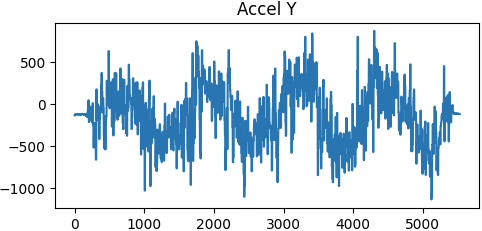
\includegraphics[width = 0.7\linewidth]{Figures/NoFilter.png}
    \caption{Nefiltrovaný signál.}
    \label{fig:NoFilter}
    \vspace{-10pt}
\end{figure}

\begin{figure}[!h]
    \centering
        \subfloat[Klouzavý průměr]{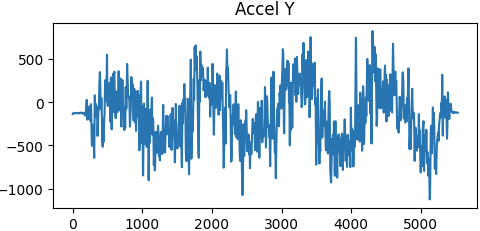
\includegraphics[width = .5\textwidth]{Figures/MovingAverage.png}\label{fig:MovingAverage}}
	    \subfloat[Jednopólová dolní propust]{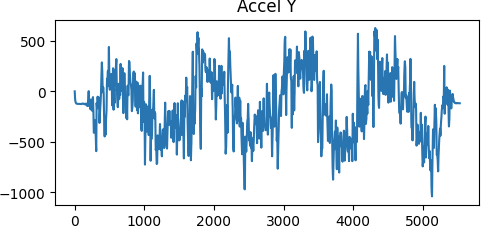
\includegraphics[width = .5\textwidth]{Figures/SinglePole.png}\label{fig:SinglePole}} \\
        \subfloat[Čtyřstupňová dolní propust]{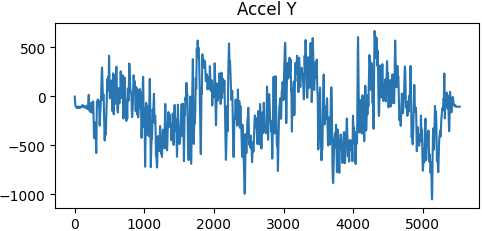
\includegraphics[width = .5\textwidth]{Figures/FourStage.png}\label{fig:FourStage}}
    	\subfloat[Dvoupólový Čebyševův filtr]{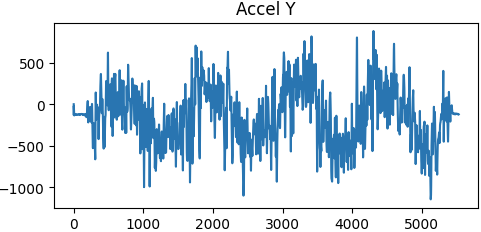
\includegraphics[width = .5\textwidth]{Figures/Chebyshev.png}\label{fig:Chebyshev}}
    \caption{Ukázky aplikovaných filtrů.}
    \label{fig:filters}
\end{figure}

Po analýze výsledků jsem dospěl k~závěru, že nejlepší výsledky ukazují filtry
\uv{Jednopólová dolní propust} a~\uv{Čtyřstupňová dolní propust}. První zmíněný byl použit pro
implementaci kvůli nejlepší redukce šumu.
\endinput
